
\paragraph{UC-10 Visualizzazione delle stanze registrate nel sistema}
\begin{itemize}
    \item \textbf{Attore primario:} amministratore;
    \item \textbf{Descrizione:} un amministratore pu\`{o} visualizzare a video l'insieme delle stanze registrate nel sistema;
    \item \textbf{Precondizione:} l'amministratore si trova nella pagina di visualizzazione delle stanze registrate nell'applicazione web;
    \item \textbf{Postcondizione:} l'amministratore visualizza tutte le stanze registrate all'interno del sistema;
    \item \textbf{Scenario principale:}
    \begin{enumerate}
        \item l'amministratore visualizza un elenco delle stanze precedentemente inserite nel sistema.
    \end{enumerate}
\end{itemize}

\begin{figure}[H]
    \centering
      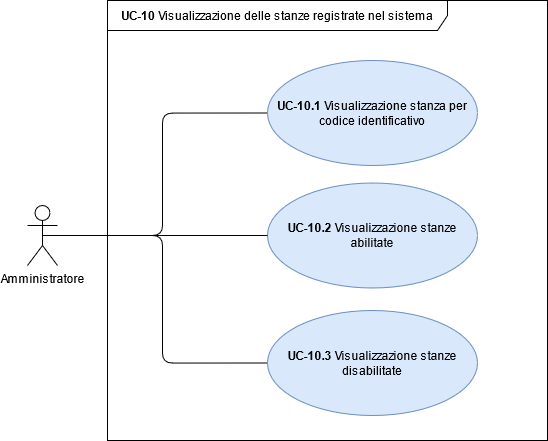
\includegraphics[scale=0.50]{src/CasiDUso/immagini/VisualizzazioneStanzeRegistrate.png}
    \caption{Diagramma relativo alla visualizzazione delle stanze registrate nel sistema}
\end{figure}


\paragraph{UC-10.1 Visualizzazione stanza per codice identificativo}
\begin{itemize}
    \item \textbf{Attore primario:} amministratore;
    \item \textbf{Descrizione:} un amministratore pu\`{o} visualizzare a video una stanza corrispondente al codice identificativo cercato;
    \item \textbf{Precondizione:} l'amministratore visualizza l'elenco di tutte le stanze registrate nel sistema;
    \item \textbf{Postcondizione:} l'amministratore ricerca la stanza tramite codice univoco identificativo. Se non esiste alcuna stanza avente codice identificativo cercato non verrà visualizzata a video alcuna stanza;
    \item \textbf{Scenario principale:}
    \begin{enumerate}
        \item l'amministratore digita il codice identificativo di una stanza da cercare nell'apposita barra di ricerca;
        \item durante la digitazione del codice identificativo vengono scremati i risultati non corrispondenti al codice cercato dall'utente ed, al termine dell'inserimento, rimarr\'{a} a video la stanza o l'insieme di stanze desiderate. Nel caso in cui non esista alcuna stanza con il codice identificativo cercato, non verrà mostrato a video alcun risultato.
    \end{enumerate}
\end{itemize}

\paragraph{UC-10.2 Visualizzazione stanze abilitate}
\begin{itemize}
    \item \textbf{Attore primario:} amministratore;
    \item \textbf{Descrizione:} un amministratore pu\`{o} visualizzare a video le stanze filtrate per uno stato attuale, ovvero abilitate al momento;
    \item \textbf{Precondizione:} l'amministratore visualizza l'elenco di tutte le stanze registrate nel sistema;
    \item \textbf{Postcondizione:} l'amministratore ricerca un insieme di stanze tramite filtro attivo. Se non esiste alcuna stanza abilitata al momento della ricerca, non verrà visualizzato alcun risultato a video;
    \item \textbf{Scenario principale:}
    \begin{enumerate}
        \item l'amministratore applica il filtro nella lista di stanze mostrate a video;
        \item una volta applicato il filtro, vengono scremati i risultati non corrispondenti al filtro stesso, e rimarranno a video solamente le stanze registrate nel sistema ed abilitate. Nel caso in cui non esista alcuna stanza con criterio corrispondente al filtro abilitato, non verrà mostrato a video alcun risultato.
    \end{enumerate}
\end{itemize}


\paragraph{UC-10.3 Visualizzazione stanze disabilitate}
\begin{itemize}
    \item \textbf{Attore primario:} amministratore;
    \item \textbf{Descrizione:} un amministratore pu\`{o} visualizzare a video le stanze filtrate per uno stato attuale, ovvero disabilitate al momento;
    \item \textbf{Precondizione:} l'amministratore visualizza l'elenco di tutte le stanze registrate nel sistema;
    \item \textbf{Postcondizione:} l'amministratore ricerca un insieme di stanze tramite filtro attivo. Se non esiste alcuna stanza disabilitata al momento della ricerca, non verrà visualizzato alcun risultato a video;
    \item \textbf{Scenario principale:}
    \begin{enumerate}
        \item l'amministratore applica il filtro nella lista di stanze mostrate a video;
        \item una volta applicato il filtro, vengono scremati i risultati non corrispondenti al filtro stesso, e rimarranno a video solamente le stanze registrate nel sistema e disabilitate. Nel caso in cui non esista alcuna stanza con criterio corrispondente al filtro abilitato, non verrà mostrato a video alcun risultato.
    \end{enumerate}
\end{itemize}


\paragraph{UC-11 Aggiunta nuova stanza nel sistema}
\begin{itemize}
    \item \textbf{Attore primario:} amministratore;
    \item \textbf{Descrizione:} un amministratore pu\`{o} aggiungere una stanza alla lista di stanze censite;
    \item \textbf{Precondizione:} l'amministratore si trova nella pagina di gestione delle stanze nell'applicazione web;
    \item \textbf{Postcondizione:} una nuova stanza \`{e} stata aggiunta alla lista di stanze disponibili;
    \item \textbf{Scenario principale:}
    \begin{enumerate}
        \item l'amministratore seleziona la funzionalità di aggiunta stanze;
        \item l'amministratore inserisce il codice identificativo della stanza (UC-11.1 Inserimento del codice di una nuova stanza);
        \item l'amministratore inserisce il codice contenuto nel tag RFID associato alla stanza (UC-11.2 Inserimento codice tag RFID);
        \item l'amministratore conferma le informazioni inserite e le salva nel sistema.
    \end{enumerate}
\end{itemize}

\begin{figure}[H]
    \centering
      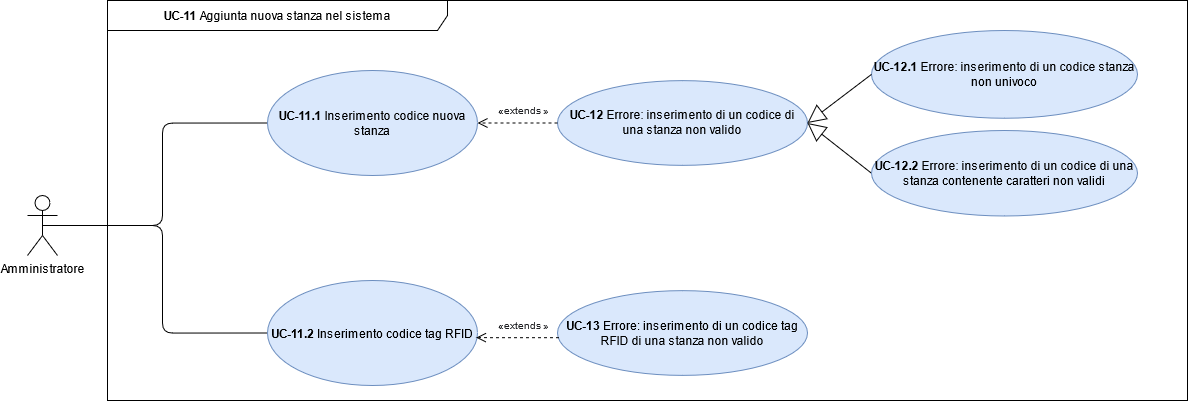
\includegraphics[scale=0.35]{src/CasiDUso/immagini/AggiuntaNuovaStanza.png}
    \caption{Diagramma relativo all'aggiunta di una nuova stanza nel sistema}
\end{figure}


\paragraph{UC-11.1 Inserimento codice nuova stanza}
   \begin{itemize}
	\item \textbf{Attore primario:} amministratore;
	\item \textbf{Descrizione:} l'amministratore vuole inserire il codice di una nuova stanza;
	\item \textbf{Precondizioni:} l'amministratore ha selezionato la funzionalità di inserimento di un codice per una nuova stanza;
	\item \textbf{Postcondizioni:} l'amministratore ha inserito con successo il codice di una nuova stanza;
	\item \textbf{Scenario principale:}
	      \begin{enumerate}
		      \item l'amministratore seleziona l'apposito box per l'inserimento del codice della nuova stanza;
		      \item il sistema controlla l'univocità del codice inserito. Qualora questa sia rispettata, elaborerà correttamente la richiesta, altrimenti mostrerà a video un messaggio di errore esplicativo (UC-12 Errore: inserimento di un codice stanza non valido).
	      \end{enumerate}
	\item \textbf{Estensioni:}
		\begin{itemize}
		      \item UC-12 Errore: inserimento di un codice di una stanza non valido.
	      \end{itemize}
\end{itemize}


\paragraph{UC-11.2 Inserimento codice tag RFID}
   \begin{itemize}
	\item \textbf{Attore primario:} amministratore;
	\item \textbf{Descrizione:} l'amministratore vuole inserire il codice tag RFID di una nuova stanza;
	\item \textbf{Precondizioni:} l'amministratore ha selezionato la funzionalità di inserimento di un codice tag RFID per una nuova stanza;
	\item \textbf{Postcondizioni:} l'amministratore ha inserito con successo il codice tag RFID di una nuova stanza;
	\item \textbf{Scenario principale:}
	      \begin{enumerate}
		      \item l'amministratore seleziona l'apposito box per l'inserimento del codice tag RFID della nuova stanza;
		      \item il sistema controlla l'univocità del codice inserito. Qualora questa sia rispettata, elaborerà correttamente la richiesta, altrimenti mostrerà a video un messaggio di errore esplicativo (UC-13 Errore: inserimento di un codice tag RFID di una stanza non valido).
	      \end{enumerate}
	\item \textbf{Estensioni:}
		\begin{itemize}
		      \item UC-13 Errore: inserimento di un codice tag RFID di una stanza non valido.
	      \end{itemize}
\end{itemize}


\paragraph{UC-12 Errore: inserimento di un codice di una stanza non valido}
\begin{itemize}
	\item \textbf{Attore primario:} amministratore;
	\item \textbf{Descrizione:} l'amministratore ha provato ad inserire il codice identificativo di nuova stanza ma l'assegnazione non è andata a buon fine poiché il codice inserito contiene dei caratteri speciali che non rispettano i criteri di inserimento;
	\item \textbf{Precondizioni:} l'amministratore ha inserito un codice identificativo errato relativo ad una stanza;
	\item \textbf{Postcondizioni:} il sistema restituisce un messaggio d'errore esplicativo e non completa l'inserimento del codice della stanza;
	\item \textbf{Scenario principale:}
	      \begin{enumerate}
		      \item il sistema elabora la richiesta ricevuta;
		      \item il sistema restituisce un messaggio d'errore esplicativo che viene visualizzato sullo schermo del dispositivo dell'amministratore e non completa la registrazione della nuova stanza.
	      \end{enumerate}
	 \item \textbf{Estensioni:}
	 	\begin{itemize}
		       \item UC-12.1 Errore: inserimento di un codice stanza non univoco;
		       \item UC-12.2 Errore: inserimento di un codice di una stanza contenente caratteri non validi.
	        \end{itemize}
\end{itemize}

\paragraph{UC-12.1 Errore: inserimento di un codice stanza non univoco}
\begin{itemize}
	\item \textbf{Attore primario:} amministratore;
	\item \textbf{Descrizione:} il sistema non permette l'assegnazione di quel nome se il codice identificativo della nuova stanza è già stato utilizzato. In tal caso viene mostrato un errore a video auto esplicativo;
	\item \textbf{Precondizioni:} l'amministratore ha inserito un codice stanza già censito nel sistema;
	\item \textbf{Postcondizioni:} il sistema restituisce un messaggio d'errore esplicativo e non completa l'inserimento della nuova stanza;
	\item \textbf{Scenario principale:}
	      \begin{enumerate}
	      	      \item l'amministratore invia i dati al sistema;
		      \item il sistema rileva una stanza già memorizzata con lo stesso codice;
		      \item il sistema restituisce un messaggio d'errore esplicativo e non permette di completare l'inserimento della nuova stanza.
	      \end{enumerate}
\end{itemize}

\paragraph{UC-12.2 Errore: inserimento di un codice di una stanza contenente caratteri non validi}
\begin{itemize}
	\item \textbf{Attore primario:} amministratore;
	\item \textbf{Descrizione:} l'amministratore ha provato ad inserire il codice identificativo di nuova stanza ma l'assegnazione non è andata a buon fine poiché il codice inserito contiene dei caratteri speciali che non rispettano i criteri di inserimento;
	\item \textbf{Precondizioni:} l'amministratore ha inserito un codice stanza che contiene dei caratteri non validi durante l'assegnazione del codice della stanza;
	\item \textbf{Postcondizioni:} il sistema restituisce un messaggio d'errore esplicativo e non completa l'inserimento della nuova stanza;
	\item \textbf{Scenario principale:}
	      \begin{enumerate}
		      \item il sistema rileva dei caratteri non validi all'interno del codice della stanza;
		      \item il sistema restituisce un messaggio d'errore esplicativo e non permette di completare l'inserimento della nuova stanza.
	      \end{enumerate}
\end{itemize}



\paragraph{UC-13 Errore: inserimento di un codice tag RFID di una stanza non valido}
\begin{itemize}
	\item \textbf{Attore primario:} amministratore;
	\item \textbf{Descrizione:} l'amministratore ha provato ad inserire il codice tag RFID di nuova stanza ma l'assegnazione non è andata a buon fine poiché il codice inserito è già censito nel sistema, quindi già associato ad una stanza esistente;
	\item \textbf{Precondizioni:} l'amministratore ha inserito un codice tag RFID di una stanza che è già censito nel sistema;
	\item \textbf{Postcondizioni:} il sistema restituisce un messaggio d'errore esplicativo e non completa l'inserimento della nuova stanza;
	\item \textbf{Scenario principale:}
	      \begin{enumerate}
		      \item il sistema rileva che il codice tag RFID inserito è già censito; 
		      \item il sistema restituisce un messaggio d'errore esplicativo e non permette di completare l'inserimento della nuova stanza.
	      \end{enumerate}
\end{itemize}

\paragraph{UC-14 Visualizzazione informazioni stanza}
\begin{itemize}
    \item \textbf{Attore primario:} amministratore;
    \item \textbf{Descrizione:} un amministratore pu\`{o} visualizzare a video tutte le informazioni disponibili per una determinata stanza selezionata;
    \item \textbf{Precondizione:} l'amministratore si trova nella pagina di gestione delle stanze nell'applicazione web;
    \item \textbf{Postcondizione:} l'amministratore visualizza tutti i dettagli della stanza selezionata, quali codice identificativo, stato postazioni ed utenti attualmente presenti al suo interno;
    \item \textbf{Scenario principale:}
    \begin{enumerate}
        \item l'amministratore visualizza un elenco delle stanze precedentemente inserite nel sistema;
        \item l'amministratore seleziona una stanza registrata nel sistema per visualizzarne le funzionalità;
        \item l'amministratore visualizza a video tutte le informazioni disponibili per la stanza selezionata, quali codice identificativo stanza (UC-14.1 Visualizzazione codice stanza), stato postazioni (UC-14.2 Visualizzazione panoramica postazioni interne ad una stanza) ed eventuali utenti presenti al suo interno (UC-14.3 Visualizzazione utenti presenti nella singola stanza).
    \end{enumerate}
\end{itemize}

\begin{figure}[H]
    \centering
      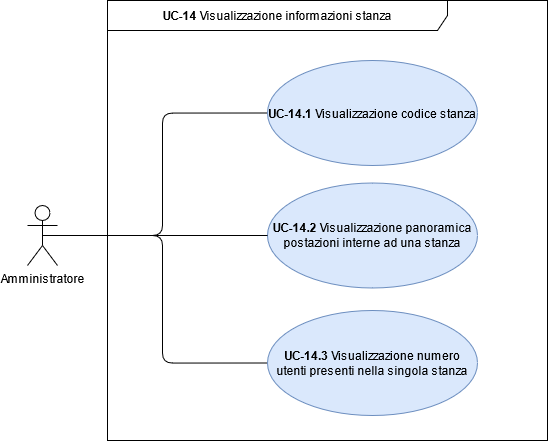
\includegraphics[scale=0.50]{src/CasiDUso/immagini/InformazioniStanza.png}
    \caption{Diagramma relativo alla visualizzazione delle informazioni di una stanza nel sistema}
\end{figure}

\paragraph{UC-14.1 Visualizzazione codice stanza}
\begin{itemize}
    \item \textbf{Attore primario:} amministratore;
    \item \textbf{Descrizione:} un amministratore pu\`{o} visualizzare a video il codice identificativo univoco di una stanza precedentemente selezionata;
    \item \textbf{Precondizione:} l'amministratore sta visualizzando a video i dettagli di una stanza selezionata;
    \item \textbf{Postcondizione:} l'amministratore visualizza il codice identificativo della stanza desiderata;
    \item \textbf{Scenario principale:}
    \begin{enumerate}
        \item l'amministratore visualizza a video il codice identificativo univoco della stanza precedentemente selezionata.
    \end{enumerate}
\end{itemize}


\paragraph{UC-14.2 Visualizzazione panoramica postazioni interne ad una stanza}
\begin{itemize}
    \item \textbf{Attore primario:} amministratore;
    \item \textbf{Descrizione:} un amministratore pu\`{o} visualizzare a video lo stato delle postazioni all'interno di una stanza precedentemente selezionata;
    \item \textbf{Precondizione:} l'amministratore sta visualizzando a video i dettagli di una stanza selezionata;
    \item \textbf{Postcondizione:} l'amministratore visualizza lo stato delle postazioni (disabilitata, occupata, sporca o libera) interne alla stanza selezionata;
    \item \textbf{Scenario principale:}
    \begin{enumerate}
        \item l'amministratore visualizza a video la lista delle postazioni interne alla stanza selezionata con, in sovrimpressione, il loro stato.
    \end{enumerate}
\end{itemize}


\paragraph{UC-14.3 Visualizzazione numero utenti presenti nella singola stanza}
\begin{itemize}
    \item \textbf{Attore primario:} amministratore;
    \item \textbf{Descrizione:} un amministratore pu\`{o} visualizzare a video il totale degli utenti presenti all'interno di una stanza precedentemente selezionata;
    \item \textbf{Precondizione:} l'amministratore sta visualizzando a video i dettagli di una stanza selezionata;
    \item \textbf{Postcondizione:} l'amministratore visualizza a video il numero di utenti presenti all'interno della stanza selezionata;
    \item \textbf{Scenario principale:}
    \begin{enumerate}
        \item l'amministratore seleziona la funzionalità di visualizzazione di tutti gli utenti presenti al momento nella singola stanza selezionata;
        \item l'amministratore visualizza a video il numero di utenti presenti all'interno della stanza selezionata.
    \end{enumerate}
\end{itemize}


\paragraph{UC-15 Visualizzazione totalità degli utenti presenti in tutte le stanze}
\begin{itemize}
    \item \textbf{Attore primario:} amministratore;
    \item \textbf{Descrizione:} un amministratore pu\`{o} visualizzare il numero di utenti presenti in tutte le stanze registrate all'interno del sistema;
    \item \textbf{Precondizione:} l'amministratore si trova nella pagina di visualizzazione delle stanze registrate nell'applicazione web;
    \item \textbf{Postcondizione:} l'amministratore visualizza il numero di utenti presenti all'interno di tutte le stanze registrate nel sistema;
    \item \textbf{Scenario principale:}
    \begin{enumerate}
        \item l'amministratore seleziona la funzionalità di visualizzazione di tutti gli utenti presenti all'interno di tutte le stanze registrate nel sistema;
        \item l'amministratore visualizza a video il numero di utenti all'interno di tutte le stanze censite nel sistema.
    \end{enumerate}
\end{itemize}

\paragraph{UC-16 Modifica codice della stanza}
\begin{itemize}
	\item \textbf{Attore primario:} amministratore;
	\item\textbf{Descrizione:} l'amministratore vuole modificare il codice univoco di una stanza;
	\item\textbf{Precondizioni:} l'amministratore accede all'apposita funzionalità di modifica dei dati di una stanza;
	\item\textbf{Postcondizioni:} l'amministratore modifica con successo il codice univoco di una stanza;
	\item \textbf{Scenario principale:}
	      \begin{enumerate}
		      \item l'amministratore visualizza un elenco delle stanze precedentemente inserite nel sistema;
		      \item l'amministratore seleziona la stanza di cui vuole cambiare il codice identificativo;
		      \item l'amministratore seleziona la funzionalità di modifica del codice identificativo per la stanza precedentemente selezionata;
		      \item l'amministratore ha modificato con successo il codice identificativo della stanza.
	      \end{enumerate}
	\item \textbf{Estensioni:}
		\begin{itemize}
		      \item UC-17 Errore: codice stanza non valido.
	      \end{itemize}
\end{itemize}

\paragraph{UC-17 Errore: codice stanza non valido}
\begin{itemize}
	\item \textbf{Attore primario:} amministratore;
	\item \textbf{Descrizione:} l'amministratore ha provato a modificare il codice identificativo di nuova stanza ma l'assegnazione non è andata a buon fine poiché il codice inserito non è univoco o contiene dei caratteri speciali che non rispettano i criteri di inserimento;
	\item \textbf{Precondizioni:} l'amministratore ha inserito un codice identificativo di nuova stanza non univoco o che contiene dei caratteri non validi durante la modifica del codice identificativo di una stanza;
	\item \textbf{Postcondizioni:} il sistema restituisce un messaggio d'errore esplicativo e non completa la modifica del codice identificativo della stanza;
	\item \textbf{Scenario principale:}
	      \begin{enumerate}
		      \item il sistema elabora la richiesta ricevuta;
		      \item il sistema restituisce un messaggio d'errore esplicativo che viene visualizzato sullo schermo del dispositivo dell'amministratore e non completa la modifica del codice identificativo della stanza.
	      \end{enumerate}
	 \item \textbf{Estensioni:}
	 	\begin{itemize}
		       \item UC-17.1 Errore: inserimento di un codice stanza non univoco;
		       \item UC-17.2 Errore: inserimento di un codice di una stanza contenente caratteri non validi.
	        \end{itemize}
\end{itemize}

\paragraph{UC-17.1 Errore: codice stanza non univoco}
\begin{itemize}
	\item \textbf{Attore primario:} amministratore;
	\item \textbf{Descrizione:} il sistema non permette l'assegnazione di quel nome se il codice identificativo della nuova stanza è già stato utilizzato. In tal caso viene mostrato un errore a video auto esplicativo;
	\item \textbf{Precondizioni:} l'amministratore ha inserito un codice stanza già censito nel sistema;
	\item \textbf{Postcondizioni:} il sistema restituisce un messaggio d'errore esplicativo e non completa l'inserimento della nuova stanza;
	\item \textbf{Scenario principale:}
	      \begin{enumerate}
	      	      \item l'amministratore invia i dati al sistema;
		      \item il sistema rileva una stanza già memorizzata con lo stesso codice;
		      \item il sistema restituisce un messaggio d'errore esplicativo e non permette di completare l'inserimento della nuova stanza.
	      \end{enumerate}
\end{itemize}
    
    
\paragraph{UC-17.2 Errore: inserimento di un codice di una stanza contenente caratteri non validi}
\begin{itemize}
	\item \textbf{Attore primario:} amministratore;
	\item \textbf{Descrizione:} l'amministratore ha provato ad inserire il codice identificativo di nuova stanza ma l'assegnazione non è andata a buon fine poiché il codice inserito contiene dei caratteri speciali che non rispettano i criteri di inserimento;
	\item \textbf{Precondizioni:} l'amministratore ha inserito un codice stanza che contiene dei caratteri non validi durante l'assegnazione del codice della stanza;
	\item \textbf{Postcondizioni:} il sistema restituisce un messaggio d'errore esplicativo e non completa l'inserimento della nuova stanza;
	\item \textbf{Scenario principale:}
	      \begin{enumerate}
		      \item il sistema rileva dei caratteri non validi all'interno del codice della stanza;
		      \item il sistema restituisce un messaggio d'errore esplicativo e non permette di completare l'inserimento della nuova stanza.
	      \end{enumerate}
\end{itemize}
 
\paragraph{UC-18 Rimozione di una stanza dal sistema}
\begin{itemize}
    \item \textbf{Attore primario:} amministratore;
    \item \textbf{Descrizione:} un amministratore pu\`{o} rimuovere una stanza dalla lista di stanze censite;
    \item \textbf{Precondizione:} l'amministratore si trova nella pagina di gestione delle stanze nell'applicazione web;
    \item \textbf{Postcondizione:} l'amministratore ha rimosso con successo una stanza dall'insieme delle stanze censite dal sistema;
    \item \textbf{Scenario principale:}
    \begin{enumerate}
        \item l'amministratore seleziona la funzionalità di rimozione stanze;
        \item l'amministratore seleziona dalla lista la stanza che desidera rimuovere;
        \item l'amministratore conferma la volontà di eliminare la stanza selezionata;
        \item l'amministratore ha eliminato con successo la stanza precedentemente selezionata dalla lista delle stanze censite all'interno del sistema.
    \end{enumerate}
\end{itemize}

\paragraph{UC-19 Disabilitazione di una stanza}
\begin{itemize}
    \item \textbf{Attore primario:} amministratore;
    \item \textbf{Descrizione:} un amministratore pu\`{o} disabilitare una stanza, impedendo la prenotazione delle postazioni presenti all'interno della stanza. Tutte le prenotazioni attive per tutte le postazioni di quella stanza vengono cancellate;
    \item \textbf{Precondizione:} l'amministratore si trova nella pagina di dettaglio della stanza nell'applicazione web;
    \item \textbf{Postcondizione:} la stanza \`{e} disabilitata, tutte le postazioni presenti all'interno della stessa non sono pi\`{u} prenotabili e le prenotazioni già effettuate vengono cancellate;
    \item \textbf{Scenario principale:}
    \begin{enumerate}
        \item l'amministratore seleziona la funzionalità di disabilitazione della stanza;
        \item le postazioni della stanza non sono pi\`{u} prenotabili;
        \item le prenotazioni delle postazioni della stanza sono cancellate.
    \end{enumerate}
\end{itemize}

\paragraph{UC-20 Riabilitazione di una stanza precedentemente disabilitata}
\begin{itemize}
    \item \textbf{Attore primario:} amministratore;
    \item \textbf{Descrizione:} un amministratore pu\`{o} abilitare una stanza precedentemente segnata come disabilitata;
    \item \textbf{Precondizione:} l'amministratore si trova nella pagina di dettaglio della stanza nell'applicazione web;
    \item \textbf{Postcondizione:} la stanza \`{e} stata abilitata e ritorna quindi fruibile agli utenti;
    \item \textbf{Scenario principale:}
    \begin{enumerate}
        \item l'amministratore seleziona la funzionalità di abilitazione della stanza precedentemente disabilitata;
        \item l'amministratore abilita nuovamente la stanza;
        \item le postazioni della stanza sono nuovamente prenotabili.
    \end{enumerate}
\end{itemize}